\documentclass[10pt]{article}
\usepackage[letterpaper,text={6.5in,8.7in},centering]{geometry}
\usepackage{amssymb,amsmath,times,url,subfigure,graphicx,theorem,alltt}
%\usepackage[pdftex,urlcolor=blue,pdfpagemode=none,pdfstartview=FitH]{hyperref}

%% url smaller font.
\makeatletter
\def\url@leostyle{%
  \@ifundefined{selectfont}{\def\UrlFont{\sf}}{\def\UrlFont{\small\ttfamily}}}
\makeatother
\urlstyle{leo}

%\usepackage[all,import]{xy}

\newcommand{\norm}[1]{\ensuremath{\left\| #1 \right\|}}
\newcommand{\abs}[1]{\ensuremath{\left| #1 \right|}}
\newcommand{\bracket}[1]{\ensuremath{\left[ #1 \right]}}
\newcommand{\braces}[1]{\ensuremath{\left\{ #1 \right\}}}
\newcommand{\parenth}[1]{\ensuremath{\left( #1 \right)}}
\newcommand{\ip}[1]{\ensuremath{\langle #1 \rangle}}
\newcommand{\refeqn}[1]{(\ref{eqn:#1})}
\newcommand{\reffig}[1]{Fig. \ref{fig:#1}}
\newcommand{\tr}[1]{\mbox{tr}\ensuremath{\negthickspace\bracket{#1}}}
\newcommand{\deriv}[2]{\ensuremath{\frac{\partial #1}{\partial #2}}}
\newcommand{\SO}{\ensuremath{\mathrm{SO(3)}}}
\newcommand{\T}{\ensuremath{\mathrm{T}}}
\newcommand{\so}{\ensuremath{\mathfrak{so}(3)}}
\newcommand{\SE}{\ensuremath{\mathrm{SE(3)}}}
\newcommand{\se}{\ensuremath{\mathfrak{se}(3)}}
\renewcommand{\Re}{\ensuremath{\mathbb{R}}}
\renewcommand{\S}{\ensuremath{\mathbb{S}}}
\newcommand{\aSE}[2]{\ensuremath{\begin{bmatrix}#1&#2\\0&1\end{bmatrix}}}
\newcommand{\ase}[2]{\ensuremath{\begin{bmatrix}#1&#2\\0&0\end{bmatrix}}}
\newcommand{\D}{\ensuremath{\mathbf{D}}}
\newcommand{\pair}[1]{\ensuremath{\left\langle #1 \right\rangle}}
\newcommand{\met}[1]{\ensuremath{\langle\!\langle #1 \rangle\!\rangle}}
\newcommand{\Ad}{\ensuremath{\mathrm{Ad}}}
\newcommand{\ad}{\ensuremath{\mathrm{ad}}}
\newcommand{\g}{\ensuremath{\mathfrak{g}}}

\renewcommand{\baselinestretch}{1.2}
\date{}

\renewcommand{\thesubsection}{\arabic{subsection}. }
\renewcommand{\thesubsubsection}{\arabic{subsection}.\arabic{subsubsection} }

\theoremstyle{plain}\theorembodyfont{\normalfont}
\newtheorem{prob}{Problem}[section]
%\renewcommand{\theprob}{\arabic{section}.\arabic{prob}}
\renewcommand{\theprob}{\arabic{prob}}

\newenvironment{subprob}%
{\renewcommand{\theenumi}{\alph{enumi}}\renewcommand{\labelenumi}{(\theenumi)}\begin{enumerate}}%
{\end{enumerate}}%


\begin{document}

\pagestyle{empty}
\section*{Circular Restricted Three-Body Problem}

\paragraph{Problem Definition}

Consider three point masses $m_1,m_2$ and $m$, acting under their mutual gravity. Assume that $m \ll m_1,m_2$, and $m_2$ is on a circular orbit around $m_1$ with orbital radius $r_{12}$. Define a reference frame $G-xyz$ such that the origin $G$ is on the mass center, and the $x$-axis points toward $m_2$. The $z$ axis is parallel to the angular momentum vector of the circular orbit, and the $y$-axis is chosen according to the rigid-handed rule. This frame is non-inertial, as it is rotating about the $z$ axis with the angular velocity $\Omega=\sqrt{\frac{\mu}{r_{12}^3}}$, where $\mu=G(m_1+m_2)$.

With respect to this frame, the masses $m_1$ and $m_2$ are fixed. Their location on the $x$ axis is given by
\begin{align*}
x_1 = -\frac{m_2}{m_1+m_2} r_{12} = -\frac{\mu_2}{\mu} r_{12},\quad 
x_2 = \frac{m_1}{m_1+m_2} r_{12} = \frac{\mu_1}{\mu} r_{12},
\end{align*}
where $\mu_1 = Gm_1$, and $\mu_2=Gm_2$.

\paragraph*{Equations of Motion} The equations of motion for the mass $m$ are given by
\begin{align}
\ddot x - 2\Omega \dot y -\Omega^2x & = -\frac{\mu_1}{r_1^3} (x-x_1)-\frac{\mu_2}{r_2^3} (x-x_2),\\
\ddot y + 2\Omega \dot y -\Omega^2y & = -\frac{\mu_1}{r_1^3} y-\frac{\mu_2}{r_2^3}y,\\
\ddot z & = -\frac{\mu_1}{r_1^3} z-\frac{\mu_2}{r_2^3}z,
\end{align}
where
\begin{align*}
\Omega=\sqrt{\frac{\mu}{r_{12}^3}},\quad r_1=\sqrt{(x-x_1)^2+y^2+z^2},\quad r_2=\sqrt{(x-x_2)^2+y^2+z^2}.
\end{align*}

\paragraph*{Lagrange Points} The above equations of motion has five fixed solution, or relative equilibria, referred to as Lagrange points. The first three Lagrange points are on the $x$-axis, and the remaining two Lagrange points are at the vertex of the equilateral triangle composed of $m_1$ and $m_2$.

\paragraph*{Jacobi Constant} Suppose that $z(0)=\dot z(0)=0$ such that $z(t)=0$ for all $t\geq 0$, i.e., we consider planar motions. Along the solution of the equations of motion, the following constant, referred to as Jacobi Constant, is fixed:
\begin{align}
C = \frac{1}{2} (\dot x^2+\dot y^2) -\frac{1}{2}\Omega^2(x^2+y^2)-\frac{\mu_1}{r_1}-\frac{\mu_2}{r_2}.\label{eqn:JC}
\end{align}
For a given initial condition $(x(0),y(0),\dot x(0),\dot y(0))$, we can compute the corresponding Jacobi constant. Then, \refeqn{JC} yields the following constraint on the position $(x,y)$:
\begin{align}
\Omega^2(x^2+y^2) + \frac{2\mu_1}{r_1}+\frac{2\mu_2}{r_2} + 2 C \geq 0,
\end{align}
which can be used to identify the feasible region of the solution.

\clearpage\newpage

\paragraph*{Earth-Moon System} The following figure illustrates the Lagrange Points and the boundary of the feasible region for varying Jacobi constant, for the Earth-Moon system. %(\textbf{Revised: 12/4/13})

\setlength{\unitlength}{0.1\textwidth}
\begin{figure}[h!]
\centerline{\small
\begin{picture}(9,9)(-0.2,0)
\put(0,0){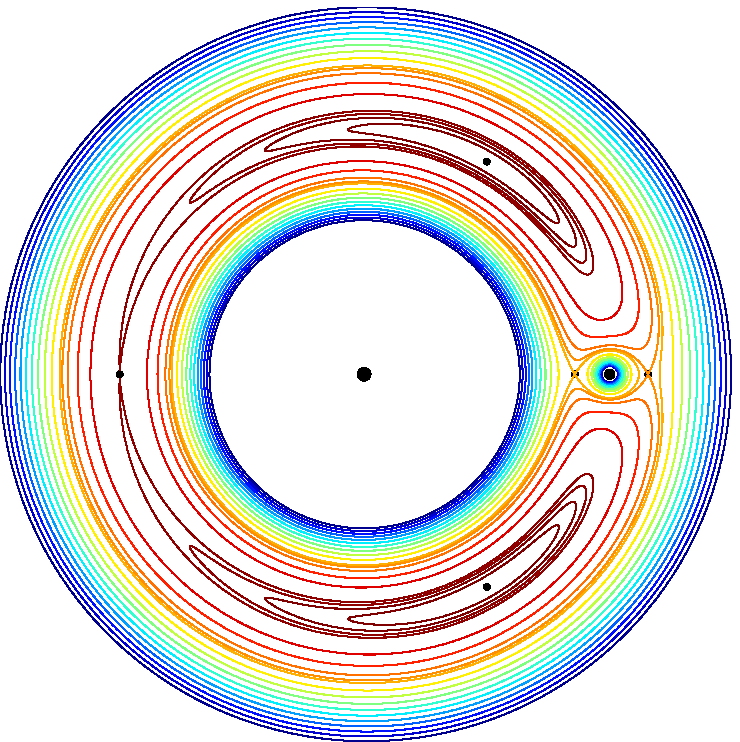
\includegraphics[width=0.8\textwidth]{JC.pdf}}
\put(1.05,3.75){$L_3$}
\put(6.05,3.75){$L_1$}
\put(7.05,3.75){$L_2$}
\put(5,6.2){$L_4$}
\put(5,1.75){$L_5$}
\end{picture}}
\end{figure}


\clearpage\newpage

\begin{figure}
\centerline{
\subfigure[$C=C_1$]{\small\setlength{\unitlength}{0.05\textwidth}
\begin{picture}(9,9)(-0.2,0)
\put(0,0){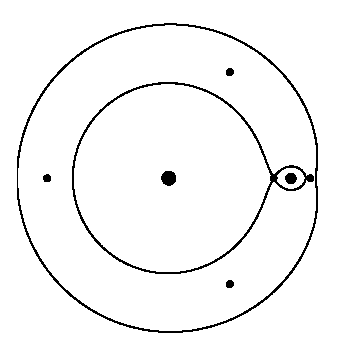
\includegraphics[width=0.4\textwidth]{R3BP_curves_1}}
\put(0.92,3.75){$L_3$}
\put(5.8,3.75){$L_1$}
\put(7.5,3.75){$L_2$}
\put(5,6.0){$L_4$}
\put(5,1.4){$L_5$}
\end{picture}}
\subfigure[$C=C_2$]{\small\setlength{\unitlength}{0.05\textwidth}
\begin{picture}(9,9)(-0.2,0)
\put(0,0){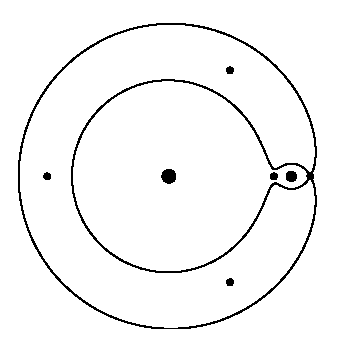
\includegraphics[width=0.4\textwidth]{R3BP_curves_2}}
\put(0.92,3.75){$L_3$}
\put(5.8,3.75){$L_1$}
\put(7.5,3.75){$L_2$}
\put(5,6.0){$L_4$}
\put(5,1.4){$L_5$}
\end{picture}}}
\centerline{
\subfigure[$C=C_3$]{\small\setlength{\unitlength}{0.05\textwidth}
\begin{picture}(9,9)(-0.2,0)
\put(0,0.4){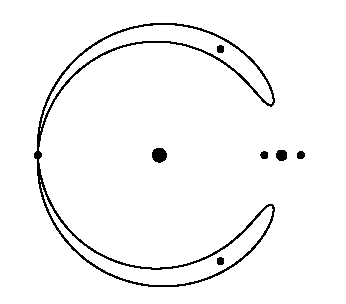
\includegraphics[width=0.4\textwidth]{R3BP_curves_3}}
\put(0.92,3.75){$L_3$}
\put(5.8,3.75){$L_1$}
\put(7.5,3.75){$L_2$}
\put(5,6.0){$L_4$}
\put(5,1.4){$L_5$}
\end{picture}}
\subfigure[$C=C_{4,5}$]{\small\setlength{\unitlength}{0.05\textwidth}
\begin{picture}(9,9)(-0.2,0)
\put(0,0.4){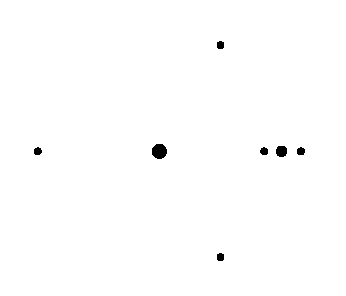
\includegraphics[width=0.4\textwidth]{R3BP_curves_5}}
\put(0.92,3.75){$L_3$}
\put(5.8,3.75){$L_1$}
\put(7.5,3.75){$L_2$}
\put(5,6.0){$L_4$}
\put(5,1.4){$L_5$}
\end{picture}}}

\end{figure}
\end{document}

